\documentclass[10pt,a4paper]{book}
\usepackage[utf8]{inputenc}
\usepackage[french]{babel}
\usepackage[T1]{fontenc}
\usepackage{amsmath}
\usepackage{amsfonts}
\usepackage{amssymb}
\usepackage{graphicx}
\author{ Antoine Robin}
\title{Warhammer - campagne}
\newcommand{\nomadversaire}{culte inconnu}
\begin{document}
\maketitle
\tableofcontents
\chapter{Arcs narratifs}
\section{Arc principal : l'influence du chaos}
Au cours de cette campagne, les PJs vont affronter l'influence pernicieuse, mais subtile d'un culte du chaos, jusqu'au déclenchement de ses plans machiavéliques.
\subsection{Synopsis}
 C'est un arc narratif en trois actes : lors du premier, les actes du culte seront très subtils, plus une menace de fond. Lors du second, les personnages auront été mis au courant de l'existence du culte, et pourront plus précisément enquêter à ce sujet. Enfin, lors du troisième, le culte se sentant menacé, va déclencher un plan plus important pour semer le chaos.
\subsection{\nomadversaire}
 
\subsection{Acte 1 : une présence discrète}
Cet acte sera assez flou, peu de vrai structure. En effet, il s'agit de plans et d'actions du culte que les personnages pourraient rencontrer, mais sans forcément voir le point commun.

La première rencontre des personnages avec le culte, même s'ils n'en auront pas conscience immédiatement, est le bailli, qui assiste les forces du chaos dans la région en leur donnant des informations, et obéi à ses maîtres de la secte. En particulier, il a guidé les récentes attaques, et a reçu l'ordre de faire sacrifier quelqu'un d'important aux dieux noirs, afin d'apporter la faveur des dieux sombres sur les envahisseurs. Après une embuscade échouée à cause des PJs(session 3), il a donc fait enlever la Ritterin von Hauptberg, et l'a livrée aux créatures de la forêt, qui s'apprêtent à la sacrifier. Il s'agira d'un combat livré à la lueur des torches, près d'une pierre de sacrifice, apparemment certains plutôt récents. Une fois ce péril vaincu, les personnages gagneront ??? PX.
\subsection{Acte 2 : un culte mystérieux}
Cet acte commence quand les personnages sont mis au courant de l'existence de ce culte, et peuvent commencer à relier les points entre certains problèmes de l'acte 1. Cela va permettre aux PJs d'enquêter beaucoup plus spécifiquement, d'après les indices qu'ils ont pu obtenir, et qu'on a pu leur donner le cas échéant.
\subsection{Acte 3 : le plan machiavélique}
Suite à l'enquête des PJs, et leur lutte contre \nomadversaire, ce culte se sent menacé, et commence à réagir beaucoup plus violemment : il ordonne la mort des PJs et commence à déclencher son plan global. Cela va amener les PJs à voyager dans l'empire pour lutter contre le coeur du culte.
\section{Arcs secondaires}
\subsection{Les marais de Schadensumpf}
Ces marais, difficiles d'accès, sont remplis de créatures et de problèmes, et les PJs pourraient avoir plusieurs raisons de s'y diriger : explorer des pistes pour enquête, chercher une ancienne relique perdue.... Au nord de ces marais, les collines embrumées, qui peuvent également receler des intérêts.
\subsection{Familles criminelles}
Trois groupes criminels sont rivaux dans la ville de Waldenheim et ses environs immédiats. L'un gère essentiellement les docks, l'autre ce qui se passe dans les faubourgs de la ville, au sud des remparts, et enfin, le troisième défend son territoire près du marché à l'ouest de la ville. En plus de leur rivalité latente, il peut y avoir des problèmes plus importants
\subsection{Sous Waldenheim}
La forteresse du clan Volkn, des skavens, se trouve sous la région, et des groupes d'éclaireurs et de pillards peuvent rôder dans le coin. En particulier, les PJs pourraient se retrouver face à ces différents groupes, ou se mettre en travers du chemin du chef de guerre du clan, Skarrik tranche-pattes.
\subsection{Les familles von Hauptberg et Oberstein}

Deux familles importantes de Waldenheim, qui sont régulièrement en conflit sur de nombreux sujets. Aujourd'hui les Oberstein ont le titre de comtes de Waldenheim, et les von Hauptberg font parti de la noblesse importante de la région, et sont une épine permanente dans leur flanc.

Les personnages pourraient sans doute être recrutés dans la maisonnée de l'une ou l'autre de ces familles, ce qui pourrait fournir de nombreuses occasions de découvrir les lieux et de travailler.

Une option est de faire rencontrer un membre d'une des maisons dans la première mission, qui pourrait leur proposer un travail.

Plus tard, le conflit entre les deux familles peut s'envenimer : duels de justice (truqués), affrontements plus ou moins violents, et une tentative d'assassinat (perpétrée par une autre faction ?). Bref, les personnages ne devraient pas trop manquer de travail à accomplir pour leur patron.

L'espionnage est une possibilité, avec la corruption d'un PJ pour obtenir des informations par un autre de leurs contacts.

\subsection{Le rassemblement de la horde}
Vaguement soutenu par les forces du culte, et profitant des trainards de la horde d'archaon, Morghast le désosseur commence à se tailler un nom dans la région : il commence à rassembler des créatures de tout type et de toute forme dans la Drakwald, sous sa bannière corrompue.

Celles-ci vont menacer les villages de la région, notamment Utingen, et formeront un adversaire adequat pour le début de campagne, avant que les PJs ne tuent leur seigneur dans un affrontement violent. 

Un arc en plusieurs parties : une partie sous la menace de la horde, une course avec celle-ci pour un lieu ou artefact, et enfin, une recherche du seigneur de la horde pour le tuer.
\section{Arcs personnels}
\subsection{Linlorryn de Laurelorn :La chasse}
un bestigor est responsable de plusieurs problèmes pour l'elfe du groupe, et les PJs pourront entendre parler de lui, voir le traquer dans la drakwald.
Il porte un symbole de crâne écarlate, et dispose d'une stature peu commune.

Ambitions :
\begin{description}
\item[Court terme :]traquer et tuer l'homme-bête responsable de ses problèmes
\item[Long terme :]Eliminer les hommes-bêtes de la Drakwald (attention !)
\end{description}
\subsection{Aldemar von Schluchenbar : L'ancienne famille}
le famille du cavalier est de petite noblesse, qui a perdu au fil du temps ses possessions et titres, ce qui l'a mené lui à monter les rangs 'à la main' plutôt que pouvoir devenir officier. Il serait peut-être possible de redorer le blason de la famille, notamment en retrouvant leurs archives, dispersées après la vente de leur domaine.

Ambitions :
\begin{description}
\item[Court terme :]faire écrire une chanson sur ses exploits
\item[Long terme :]obtenir une reconnaissance impériale
\end{description}
\subsection{Unduk Umberbuckelesson Unboki La mort glorieuse}
le tueur cherche à mourir, ce qui devrait être possible : penser à inclure une galerie de créatures de plus en plus grosses à tuer, permettant de trouver une fin glorieuse. Hommes-bêtes, trolls, guerriers du chaos, minotaure, démons .....

Ambitions :
\begin{description}
\item[Court terme :]Pacifier un adversire plus grand que lui
\item[Long terme :]mourir
\end{description}
\subsection{Nelis van Egelen :Connaissances interdites}
l'érudit du groupe est suivi par les chasseurs de sorciers, qui le suspectent d'avoir certaines connaissances interdites. Il les a fuit pour éviter leur sinistre réputation. Il est peut-être possible de travailler avec eux ou de les convaincre de la bonne foi du personnage. Dans ce cas, ils pourraient devenir des alliés, ou sinon, se révéler être des problèmes récurrents.

Ambitions :
\begin{description}
\item[Court terme :]atteindre Altdorf. A voir, peut-être inclure un groupe de mages à Waldenheim, qui pourraient être convaincus.
\item[Long terme :]découvrir les origines des vents de magie (interdit ! :p)
\end{description}
\subsection{Johannes Kleinman : des relations compliquées}
bâtard de la famille von Hauptberg, en rivalité avec les comtes de Waldenheim.

A reçu la consigne de laisser passer des voyageurs ayant un écusson représentant une main squelettique (un des groupes criminels de Waldenheim).

Ambitions :
\begin{description}
\item[Court terme :]???
\item[Long terme :]???
\end{description}
\section{Arcs tertiaires}
\subsection{Une menace sur le village}
Cet arc va ouvrir la campagne, en proposant une enquête/traque.

Le Bailli du village voit les personnages arriver, et souhaite leur proposer un travail : depuis quelques temps, les bois grouillent de créatures dangereuses, et il souhaiterai, si possible, que les aventuriers aillent vérifier ce dont il s'agit. En particulier, le meunier a affirmé que des créatures rôdent près de chez lui.

En effet, des hommes-bêtes cherchent des victimes à tuer dans la région, et le moulin, un des bâtiments les plus visibles de la région, attire facilement leur convoitise.

Cela peut se traduire par une première attaque par des ungors, qui voyaient cela comme une cible facile. Leurs traces peuvent ensuite être remontées vers une petite grotte voisine, ou une troupe un peu plus importante fait rôtir une bête quelconque. Si les traces ne peuvent être suivies, des rumeurs sur la 'vieille caverne', où des charbonniers auraient entendu des bruits étranges et vus des traces inquiétantes.

Les aventuriers vont pouvoir se rendre compte de la présence d'un symbole commun sur plusieurs des adversaires vaincus, une sorte de crâne hurlant écarlate, que l'asrai pourra sans trop de problème identifier.
\subsection{Nuit sanglante (Aventure commerce)}
Peut arriver sur tout trajet des PJs sur une route.

Alors que les personnages sont forcés de s'abriter dans une petite auberge par une tempête, un groupe de cultistes de Tzeentch vient de s'en emparer, et prépare une cérémonie pour sacrifier ses anciens occupants. Des PJs peu suspicieux pourront sans mal être ajoutés à celle-ci, et satisfaire leur seigneur noir.
\subsection{ça a le goût de poulet}
Un riche marchand de Marienburg est récemment arrivé en ville, et cherche à manger des plats locaux, en particulier les viandes qu'il n'aurait jamais testé auparavant. Les aubergistes de Waldenheim sont ravis de lui faire goûter leurs spécialités, mais les citadins commencent à rapporter des disparitions, et beaucoup sont persuadés que ce marchand en est la cause : ce serait un cannibale !

Quand les personnages arrivent pour s'en débarrasser, payés par la populace, ils découvrent son corps, comme mangé de l'intérieur par quelque chose d'innommable. Pour beaucoup d'habitants, les PJs sont alors coupables des disparitions ! Les personnages vont devoir trouver rapidement la cause du problème avant d'être lynchés.
\chapter{Déroulement de la campagne}
\section{Acte 1 : un complot discret}
La campagne débutera dans le village d'Utingen, un petit village fortifié le long de la route du nord. Celui-ci a récemment été l'objet de raids d'hommes-bêtes, peu nombreux, mais dangereux. Et le bailli a eu vent de la présence de potentiels aventuriers dans son village, et va essayer de les convaincre de lui donner un coup de main, contre monnaie sonnante et trébuchante. \emph{Arc tertiaire : une menace sur le village.} A priori, il ne devrait pas y avoir d'autre lien avec les autres arcs, mais peut-être l'inclure discrètement dans un butin, ou autre. 

Alors que les aventuriers auront vaincu un petit groupe d'hommes-bêtes, ils vont entendre des bruits plus importants au loin : des cornes résonnent dans la forêt, ce qui n'est jamais bon signe. Quand ils reviennent au village, le bailli, Dieter Wolfensohn, les récompense et entendant les nouvelles, semble s'alarmer, et leur demande s'ils peuvent rester aider à défendre le village. En acceptant, ils se retrouvent rapidement à affronter un groupe d'avant-garde. Celui-ci vaincu, les villageois vont leur demander de l'aide, une escorte jusqu'à Waldenheim.

Lors de ce trajet, plusieurs éléments devraient arriver:
\begin{itemize}
\item première rencontre avec le culte (nom et détails à trouver !) : le bailli du village est un traître, qui va essayer de faire tomber le groupe dans un piège, puis, en cas d'échec, va monter les villageois contre les PJs. (arc principal)
\item rencontre avec la famille von Hauptberg, en passant par leur manoir. La Riterrin Anna von Hauptberg rejoindra d'ailleurs le convoi, et sera ainsi aussi en danger. Dans sa suite se trouve aussi un artiste, qui a récemment dû quitter Altdorf précipitament (arcs de Johannes et Aldemar)
\item Linlorryn devrait se rendre compte de la présence d'un symbole qu'elle connait/reconnait bien : le bestigor ! (arc le linlorryn)
\end{itemize}

La première tentative du bailli va consister à proposer un 'raccourci' menant au manoir de la Ritterin, un peu plus difficile à traverser, mais permettant de gagner plusieurs heures. Evidemment, au milieu de celui-ci, un groupe d'hommes-bêtes va tenter de s'attaquer aux villageois.

La seconde tentative du bailli sera plus osée : il va devoir d'abord sortir du convoi pour aller chercher ses alliés maléfiques, pour tenter d'enlever la ritterin au milieu de la nuit. Les personnages à leur poursuite finiront peut-être par tomber sur la pierre de sacrifice, autour de laquelle s'affaire un shaman homme-bête, ainsi que quelques autres créatures. La Ritterin von Hauptberg doit bientôt être sacrifiée, avec d'autres prisonniers.

La troisième tentative, si elle est possible, sera de rassembler les villageois contre les PJs pour essayer de les lyncher. Il va pendant un certain temps râler sur ces étrangers qui sont arrivés et à cause de qui tout  va mal. A une demi-journée de Waldenheim, il pourra tenter de transformer les villageois en horde acharnée.

Suivant l'efficacité des PJs, plusieurs résultats sont possibles:
\begin{itemize}
\item La Riterrin peut être encore en vie, probablement avec une certaine reconnaissance pour les PJs. Elle pourrait alors leur proposer un emploi au sein de sa maisonnée.
\item Le bailli pourrait avoir été démasqué, ce qui leur ferait dors et déjà une petite réputation, et leur donnerait un premier indice de la présence d'un culte dans la région : il porte sur lui un des symboles de celui-ci, sous la forme d'un tatouage.
\item Le bestigor honni pourrait avoir été vaincu, au cours des affrontements. Dans ce cas, l'elfe va pouvoir marginalement se calmer.
\end{itemize}
\chapter{Dramatis personae}
\section{Dans la Drakwald}
Ritterin Anna von Hauptberg : noble impériale
Griselda Werdin : guérisseuse
Dieter Wolfensohn : bailli
Berthold Sternberg : ancien militaire, amant de la riterrin.
\section{A Waldenheim}
\section{Le reste de l'empire}

\chapter{Lieux importants}
\section{Waldenheim}
Waldenheim est une ville relativement fortifiée à la frontière entre le middenland, le nordland et les désolations de Marienburg. Elle appartient au Middenland.

Elle protège l'entrée de la grande route du nord dans la Drakwald.
\section{Utingen}
Un petit village à environ deux jours de marche de Waldenheim, dans la Drakwald, à proximité immédiate de la vieille route du nord. 

Il s'agit de quelques habitations regroupées autour de champs, un moulin est à un peu plus d'une heure de marche, le long d'une rivière dans la forêt. 

Pour les gens de passage, le principal intérêt du village est son auberge, le crâne bleu : elle est relativement sûre et la nourriture et les boissons sont tout à fait correctes.
\chapter{Profils utilisés}
\section{Adversaires}

\chapter{Résumés de session}
\section{Session 0}
Création des personnages. On a le groupe au début de campagne :
\begin{itemize}
\item Un tueur nain
\item Un cavalier impérial
\item Une chevalière elfe
\item Un garde humain
\item Un érudit humain.
\end{itemize}
A priori le groupe se sera formé un peu au hasard de la route vers Waldenheim.
\section{Session 1}
\paragraph{Date :}05.12.2020
\paragraph{Présents} Tout le monde.

\paragraph{Notes de séances}
Les personnages se rencontrent au crâne bleu, après être arrivés à Utingen, et parlant à l'aubergiste apprennent que des créatures auraient été aperçues dans les environs. Urduk y voit une occasion rêvée, rapidement suivi par Lindoryn et Aldemar. Nelis est embarqué plus ou moins de force par le tueur, et le garde rejoint le groupe car il connait la région mieux que les 4 autres.

Le groupe se met ensuite en route vers le moulin, où les créatures auraient été aperçues, et trouvent rapidement des traces de pas.

Ils tombent en milieu de journée sur un groupe d'hommes-bêtes pour leur premier combat, et les tuent sans trop de soucis dans une clairière de la Drakwald, marquée par un grand arbre détruit en son centre (rien de spécial, mais ça fait classe).

xp donné : 100 pour tout le monde, 25 supplémentaire pour Urduk pour son interprétation.

\paragraph{Remarques et améliorations} 
\begin{itemize}
\item Préparer les fiches PNJs à l'avance pour gagner beaucoup de temps avec les automatismes de table
\item noter les bonus courant sur une table hors du livre
\item L'écran du MJ est très pratique
\item Les tokens ont fait l'unanimité, ainsi que les cartes isométriques, une utilisation à continuer en vrai :)
\item Gagner du temps en préparant mieux les cartes de rencontres en avance, mais ça reste gérable au besoin de les faire rapidement quand on a le décors adapté déjà opérationnel
\item Il faudrait peut-être trouver un système pour gérer les avantages en combat, mais le système actuel de pastille reste pas mal.
\end{itemize}
\section{session 2}
\paragraph{Date:} 03.01.2021
\paragraph{Présents:}Tous le monde
\paragraph{Notes de séance}
Les joueurs sont allés enquêter sur les bruits d'hommes-bêtes entendus dans la Drakwald, avant de combattre les abords de la harde (y compris un troll). En se repliant ensuite au village d'Utingen, ils ont informé le bailli, qui leur a demandé de rester un peu plus pour les aider à défendre le village. Village effectivement attaqué le lendemain matin. Ce premier assaut a été repoussé par les aventuriers, avec un mélange d'hommes-bêtes et de maraudeurs du chaos.
\paragraph{Remarques et améliorations}
\begin{itemize}
\item Il faudrait sérieusement mieux travailler les règles, possiblement en prenant des notes à leur sujet, et en notant les pages les plus utiles : critiques, bonus/malus....
\item Il faudrait lancer plus l'intrigue : pour le moment le début de campagne a été plutôt aride, et mériterait un travail plus profond sur les éléments à amener ainsi que la façon de le faire. A la fin de la prochaine séance, les personnages devraient commencer à découvrir certains des problèmes de la région, et commencer à essayer de les résoudre.
\item Il faut anticiper les récompenses, que ce soit monétaires ou en xp : le temps de réflexion est trop long pour se justifier présentement.
\end{itemize}
\section{session 3}
\paragraph{Date:} 17.01.2021
\paragraph{Présents:}Tous le monde
\paragraph{Notes de séance} L'équipe a accepté de rejoindre les villageois qui fuient vers Waldenheim, en faisant un détour pour prévenir et demander conseil à la ritterin von Hauptberg. Celle-ci rejoint la caravane, qui part. Le bailli réalise sa première tentative d'attaque, en menant le convoi droit dans une embuscade. Après l'échec de celle-ci, il enlève la ritterin au cours de la nuit, évènement sur lequel la séance s'est terminé, alors que Linlorryn a trouvé des traces de lutte, et d'hommes-bêtes ! Les personnages ont reçu 125xp, ainsi que des bijoux ayant une certaine valeur (pas encore estimés, un anneau masculin, et un collier féminin).
\paragraph{Remarques et améliorations}
Il faudrait surtout trouver les tokens pour les PNJs utile pour la prochaine fois, notamment ici l'herboriste ainsi que la ritterin, qui étaient prévues, mais pour lesquelles aucun token n'a été pris.
\section{Session 4 : Hexennacht}
\paragraph{Date}08.02.2021
\paragraph{Présents} Tous le monde
\paragraph{Notes de séance}
Les personnages ont suivi les traces des hommes-bêtes ayant enlevés la Ritterin von Hauptberg, jusqu'à une pierre de sacrifice dans les profondeurs de la Drakwald, alors que Morrslieb étendait sa lueur malsaine sur le monde.

Le shaman homme-bête, ainsi que les gors à proximité furent aisément vaincus, ainsi que le bailli, alors qu'il tentait de fuir. La Ritterin fut ainsi sauvée. Linlorryn a reconnu le symbole du bestigor qu'elle traque sur le shaman, et va sans doute continuer à traquer cette harde. Les PJs ont noté un tatouage étrange sur le corps du bailli, le symbole du culte auquel il appartient. Ils ont aussi trouvé une carte, marquant l'emplacement probable de la harde.

La séance s'est terminée avec l'arrivée du convoi en vue des murs de Waldenheim. Idéalement, entre cette séance et la suivante, le temps hors aventure devrait être géré par discord. Les perosonnages ont tous reçus 200xp pour la fin de cette première aventure.

\paragraph{Remarques}
Cela aurait été une bonne idée de revoir les règles de magies plus en détail avant la séance pour être plus opérationnel à leur sujet. De même, une fiche roll20 aurait été la bienvenue pour le shaman.

Il va falloir gérer le temps hors aventure sur le discord pour gagner du temps, et notamment décider avec les joueurs de leurs avancements et récompenses.
\chapter*{annexe}
\section{Carte des lieux}
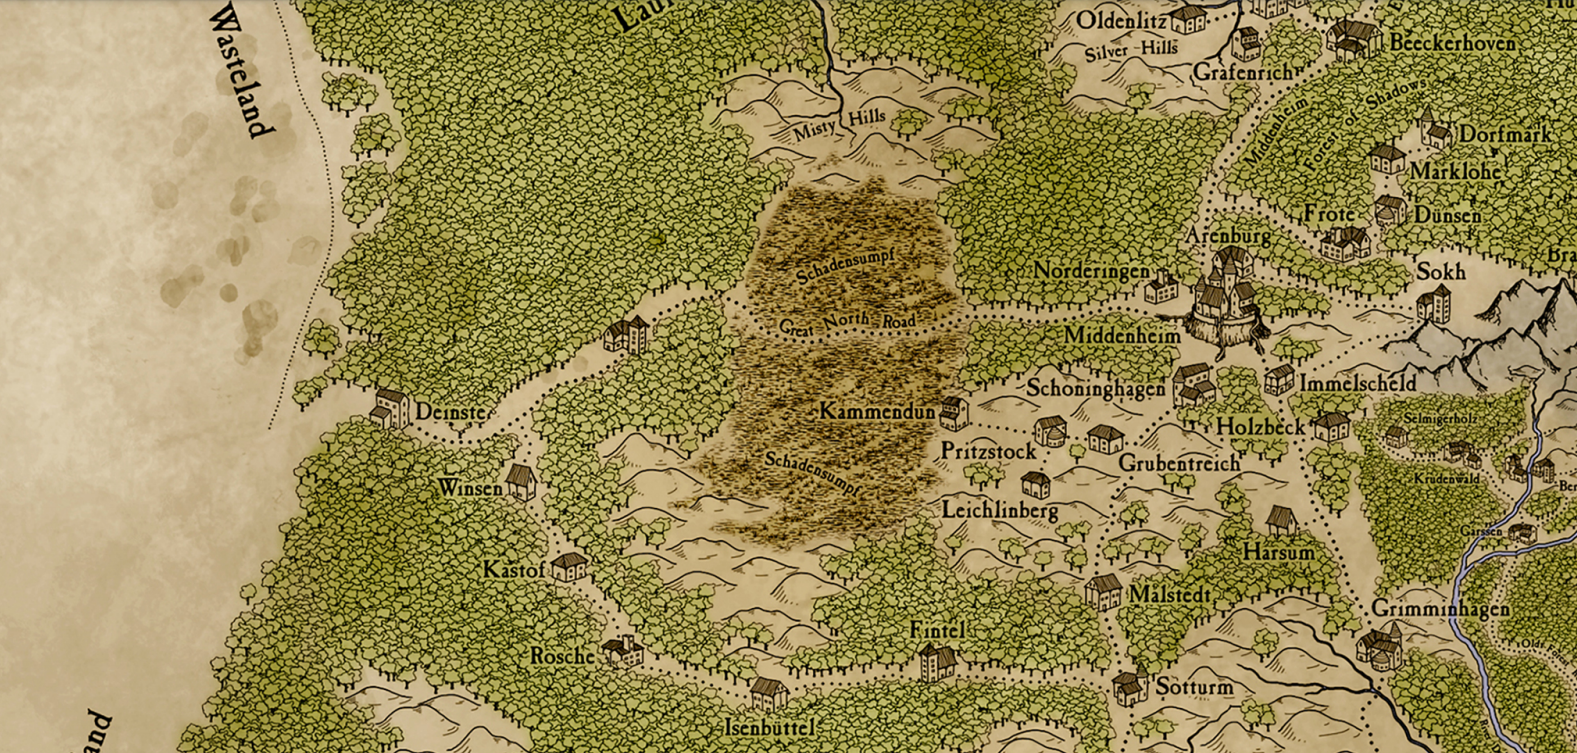
\includegraphics[width=\textwidth]{carte locale.png}
\end{document}